\subsection{YOLO模型简介}

% \begin{figure}[H]
%     \centering %表示居中
%     \includegraphics[height=8cm]{../YOLO/pics/img1.png}
%     \caption{YOLOv8架构}
% \end{figure}

\begin{wrapfigure}{r}{0.45\textwidth}
    \centering %表示居中
    \includegraphics[height=7cm]{../../YOLO/pics/img1.png}
    \caption{YOLOv8架构}
\end{wrapfigure}

YOLO模型有很多版本,本文章使用的是较新的YOLOv8\footnote{YOLOv8的详细信息可以从https://github.com/ultralytics/ultralytics处获取。}模型。

通过架构图,对比之前的 YOLO 模型,YOLOv8 主要进行了一下改动: \par
1. 提供了一个全新的 SOTA 模型,包括 P5 640 和 P6 1280 分辨率的目标检测网络和基于 YOLACT 的实例分割模型。
和 YOLOv5 一样,基于缩放系数也提供了 N/S/M/L/X 尺度的不同大小模型,用于满足不同场景需求。 \par
2. 骨干网络和 Neck 部分可能参考了 YOLOv7 ELAN 设计思想,将 YOLOv5 的 C3 结构换成了梯度流更丰富的 C2f 结构,并对不同尺度模型调整了不同的通道数,属于对模型结构精心微调,不再是无脑一套参数应用所有模型,大幅提升了模型性能。
不过这个 C2f 模块中存在 Split 等操作对特定硬件部署没有之前那么友好了。\par
3. Head 部分相比 YOLOv5 改动较大,换成了目前主流的解耦头结构,将分类和检测头分离,同时也从 Anchor-Based 换成了 Anchor-Free。\par
4. Loss 计算方面采用了 TaskAlignedAssigner 正样本分配策略,并引入了 Distribution Focal Loss。\par
5. 训练的数据增强部分引入了 YOLOX 中的最后 10 epoch 关闭 Mosiac 增强的操作,可以有效地提升精度。\par


\begin{figure}[H]
    \centering %表示居中
    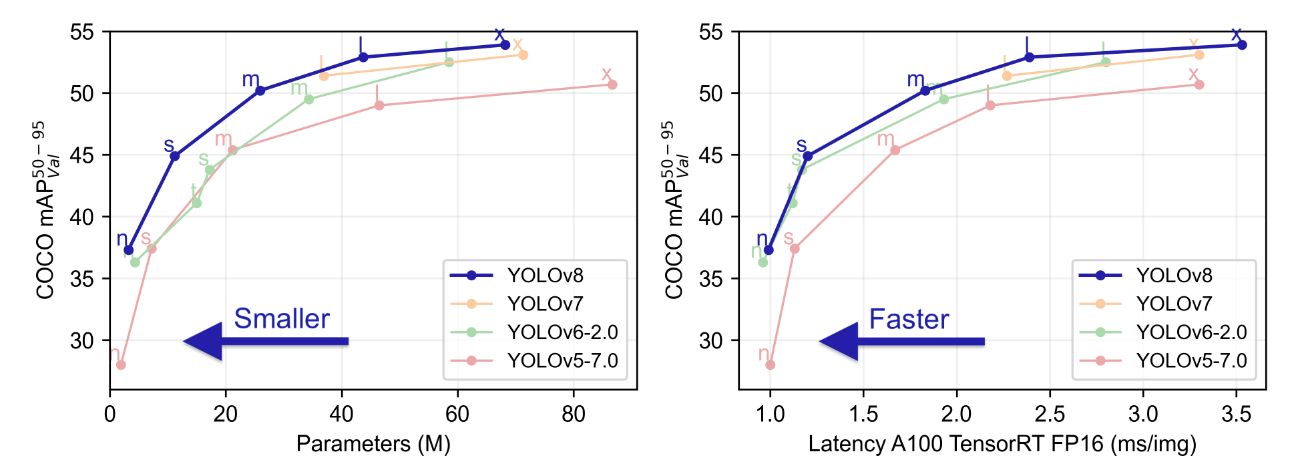
\includegraphics[height=4.5cm]{../../YOLO/pics/img.png}
    \caption{历代YOLO对比}
\end{figure}


\subsection{使用YOLO模型对图像进行识别的效果分析}